\documentclass[12pt]{article}
\usepackage[utf8]{inputenc}
\usepackage{amsmath,amssymb,latexsym}
\usepackage{enumerate}
\usepackage{graphicx}
\usepackage{float}
\usepackage[spanish]{babel}
\usepackage{xypic}

\textheight=25cm \textwidth=18cm \topmargin=-2cm \oddsidemargin=-1cm

\newcommand{\abs}[1]{\left\vert#1\right\vert}
\newcommand{\norm}[1]{\left\Vert#1\right\Vert}

\newcommand{\Co}{\mathfrak C}
\newcommand{\diag}{\mathrm{diag}}
\newcommand{\Ext}{\mathrm{ext}}
\newcommand{\F}{\mathfrak F}
\newcommand{\h}{\mathrm h}
\newcommand{\Int}{\mathrm{int}}
\newcommand{\n}{\mathfrak{n}}
\newcommand{\N}{\mathbb N}
\newcommand{\Q}{\mathbb Q}
\newcommand{\R}{\mathbb R}
\newcommand{\US}{\mathbb{S}^2}
\newcommand{\x}{\mathrm x}
\newcommand{\xk}{(\x_k)_{k\in \N}}
\newcommand{\y}{\mathrm y}
\newcommand{\z}{\mathrm z}
\newcommand{\Z}{\mathbb Z}

\newcommand{\eps}{\varepsilon}
\newcommand{\lbil}{\left <}
\newcommand{\rbil}{\right >}
\newcommand{\To}{\longrightarrow}
\newcommand{\mTo}{\longmapsto}

\begin{document}

\pagestyle{empty}
\begin{center}
{\textsc{Cálculo Diferencial e Integral III} \\
\medskip 
\large{Ejercicios I - 2 \\
Luis David Uicab Martínez \\
(Funciones entre espacios euclidianos)}}
\end{center}
\bigskip

\begin{enumerate}

\item Supongamos que $L:\R^n\To \R^m$ es una funci\'on lineal. Prueba:
\begin{enumerate}[(1)]
\item Existe $M>0$ tal que $\norm{L(\x)}\leq M\norm{\x}$ para toda 
$\x\in \R^n$.
\item si $L:\R^2\To \R$ entonces la gr\'afica de $L$ es un plano que pasa por el origen. Rec\'iprocamente, cualquier plano cuya ecuaci\'on sea de la forma $ax+by+cz=0$ con $c\neq 0$, coincide con la gr\'afica de alguna funci\'on lineal $L:\R^2\To \R$.
\end{enumerate}
\textbf{Demostración.} \\ (I) Sea $\{e_1,...,e_n\}$ la base canónica de $\R^n$. Así, para $\x=(a_1,\ldots,a_n) \in \R^n$ arbitrario, puesto que $L$ es lineal tenemos que
\[
L(\x) = L\left(\sum_{i=1}^{n}a_ie_i\right) = \sum_{i=1}^{n}a_iL(e_i).
\]
Definamos
\[
M_0=\max\{\norm{L(e_1)},\ldots,\norm{L(e_n)},1\} \text{ y } M=M_0\frac{n}{\sqrt{n}} > 0.
\]
Sea $\x$ como antes. De la desigualdad del triángulo  y la definición de  $M_0$ tenemos que
\begin{align*}
    \norm{L(\x)} &= \norm{\sum_{i=1}^{n}a_iL(e_i)} \\
    &\leq \sum_{i=1}^{n}\abs{a_i}\norm{L(e_i)} \\
    &\leq \sum_{i=1}^{n}\abs{a_i}M_0. \tag{1}
\end{align*}
Por otra parte, de la desigualdad de la media cuadrática - media aritmética y la definición de $M_0$ se sigue que
\begin{align*}
    \frac{1}{n}\sum_{i=1}^{n}\abs{a_i} \leq \sqrt{\frac{1}{n}\sum_{i=1}^{n}\left(\abs{a_i}\right)^2} &\implies \sum_{i=1}^{n}\abs{a_i} \leq \frac{n}{\sqrt{n}}\sqrt{\sum_{i=1}^{n}a_i^2}\\
    &\implies \sum_{i=1}^{n}\abs{a_i} \leq \frac{n}{\sqrt{n}}\norm{\x}\\
    &\implies M_0\sum_{i=1}^{n}\abs{a_i} \leq M_0\frac{n}{\sqrt{n}}\norm{\x}\\
    &\implies \sum_{i=1}^{n}\abs{a_i}M_0 \leq M\norm{\x}.
\end{align*}
Luego, de la desigualdad anterior, y la mencionada en $(1)$, afirmamos que
\[
\norm{L(\x)} \leq M\norm{\x}.
\]
(II) Procedamos con la suficiencia. Dada la linealidad de $L$ se tiene que
\[
L(x,y) = xL(e_1) + yL(e_2).
\]
Tomemos $L(e_1)=a$, $L(e_2)=2$ y $cz=-L(x,y)$ para alguna $c\neq 0$. Sustituyendo dichas igualdades en la ecuación previa tenemos que
\[
-cz = xa + yb \implies ax + by + cz = 0.
\]
Luego, dado que la terna $(0,0,0)$ satisface la ecuación anterior, terminamos por afirmar que dicha ecuación pertenece a un plano que pasa por el origen. \\
Sigamos con la necesidad. Sea $ax+by+cz=0$ la ecuación de un plano tal que $c\neq 0$. Tenemos entonces que
\begin{align*}
    z=-\frac{a}{c}x -\frac{b}{c}y.
\end{align*}
Definamos la función lineal $L_1$, como $L_1(e_1)=-a/c$ y $L_1(e_2)=-b/c$. En consecuencia, $L_1(x,y)=xL_1(e_1)+yL_2(e_2)$, de dónde se sigue, son expresiones equivalentes. $\blacksquare$
\newpage
\item Analiza el dominio y bosqueja la imagen de las funciones  
$\gamma:\R\To \R^n$ dadas por:
\begin{enumerate}[(1)]
\item $\gamma(t)=(t^3-t,t^2-1)$.
\item $\gamma(t)=((a\cos t,b\sen t,t)$, con $a,b>0$.
\end{enumerate}
\textbf{Solución.}
\begin{enumerate}[(1)]
    \item El dominio de $\gamma$ es todo $\R$, puesto que para todo real, la función está bien definida. Definiendo $x=t^3-t$ y $y=t^2-1$, se tiene que $\gamma(t)=(x,y)$ y $\gamma(-t)=(-x,y)$,
    de lo que afirmamos, la gráfica de la imagen de $\gamma$ está reflejada respecto al eje $y$.
    \begin{figure}[H]
        \centering
        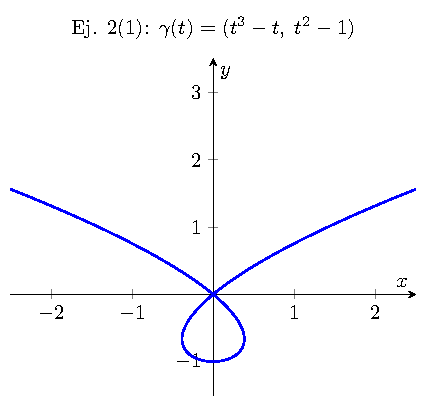
\includegraphics[width=0.4\textwidth]{Ej2 1.pdf}
    \end{figure}
    \item Puesto que $\cos t, \sen t$ están definidas para todo $t$, se sigue que el dominio de $\gamma(t)$ es todo $\R$. Hacemos notar que de ser $a=b$, la imagen de $\gamma$ es la de un círculo
    vista desde una vista paralela al plano $\Pi_{xy}$.
    \begin{figure}[H]
        \centering
        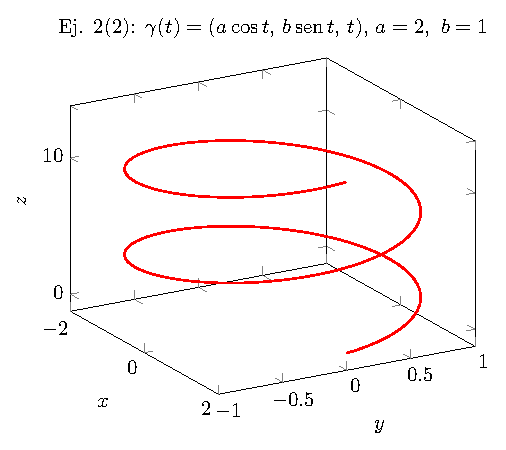
\includegraphics[width=0.4\textwidth]{Ej2 2.pdf}
    \end{figure}
    $\hfill \blacktriangle$
\end{enumerate}

\newpage
\item Determina el dominio, conjuntos de nivel y bosqueja la gr\'afica de las siguientes funciones:
\begin{enumerate}[(1)]
\item $f(x,y)=xy$.
\item $f(x,y)=x^2-y^2$.
\end{enumerate}
\textbf{Solución.}
\begin{enumerate}
    \item A priori, el dominio de $f$ es todo $\R^2$ puesto que el producto está bien definido. Procedamos a determinar los conjuntos de nivel. Si $c=0$, tenemos que
    \begin{align*}
        f^{-1}(c) &= \{(x,y)\in \R^2:xy=0\} \\
        &= \{(x,y)\in \R^2:x=0 \text{ o } y=0\} \\
        &= \{(0,y),(x,0):x,y\in \R\}.
    \end{align*}
    Sea $c>0$. Tenemos que
    \begin{align*}
        f^{-1}(c)&= \{(x,y)\in \R^2:xy>0\} \\
        &= \{(x,y)\in \R^2:x,y>0 \text{ o } x,y<0\} \\
    \end{align*}
    Si $c<0$ se sigue que
    \begin{align*}
        f^{-1}(c)&= \{(x,y)\in \R^2:xy<0\} \\
        &= \{(x,y)\in \R^2:x<0,y>0 \text{ o } x>,y<0\}.
    \end{align*}    
    De lo anterior afirmamos que la gráfica vista de forma paralela al plano $\Pi_{xy}$ se verá como un plano. Por otra parte, observando los cuadrantes $II$ y $IV$ del plano antes mencionado,
    deducimos que los puntos de la función localizados en dichos lugar son de altura negativa por como fue descrito el conjunto de nivel para $c<0$. Caso contrario para los puntos en los cuadrantes $I$ y $III$.
    Hacemos notar que el punto $(x,y,xy)$ con $f(x,y)=0$ está localizado precisamente en el origen.
    \begin{figure}[H]
        \centering
        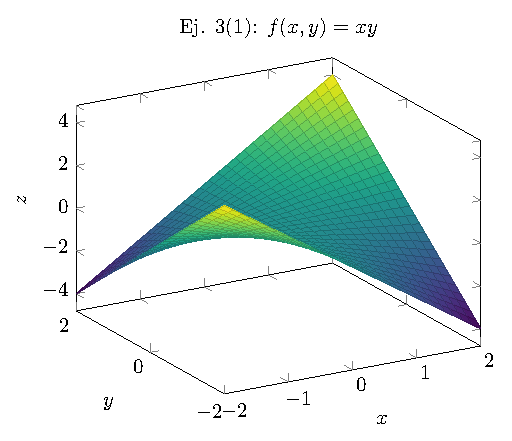
\includegraphics[width=0.4\textwidth]{Ej3 1.pdf}
    \end{figure}
    \item Al estar $f$ bien definida para todo par ordenado, afirmamos que $\text{dom}(f)=\R^2$. Notemos que, para $c=0$
    \begin{align*}
        f^{-1}(c) &= \{(x,y)\in \R^2: x^2-y^2=0\} \\
        &= \{(x,y)\in \R^2: y^2=x^2\} \\
        &= \{(x,y)\in \R^2: y=\abs{x}\}.
    \end{align*}
    Si $c>0$, tenemos que $f^{-1}(c)=\{(x,y)\in \R^2: x^2-y^2>0\}$ son los puntos correspondientes a hipérbolas horizontales. Para el caso en que $c<0$, tenemos que $x^2-y^2<0$, y en consecuencia, los puntos pertenecen a hipérbolas
    verticales.
    \begin{figure}[H]
        \centering
        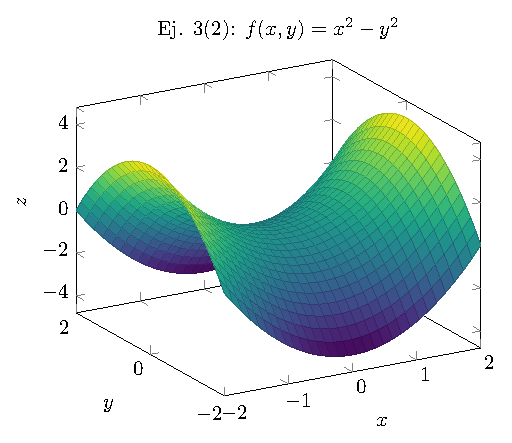
\includegraphics[width=0.4\textwidth]{Ej 3 2.pdf}
    \end{figure}
    $\hfill \blacktriangle$
\end{enumerate}

\newpage
\item Si $f(x,y)=(x^2-y^2,2xy)$, determina la imagen de los planos 
$A=\{(x,y)\in \R^2:x\geq 0, y\geq 0\}$ y $B=\{(x,y)\in \R^2:y\geq 0\}$ bajo $f$. \\
\textbf{Demostración}. Tenemos que
\begin{align*}
    f(A) &= \{f(x,y):x\in A\} \\
    &= \{(x^2-y^2,2xy):x\geq 0, y \geq 0\}.
\end{align*}
Notemos que al ser $x,y$ números no negativos, $2xy \geq 0$. Por otra parte, si $x=y$, $x^2-y^2=0$. Para $x<y$, $x^2-y^2<0$, y si $x>y$, $x^2-y^2=0$. Así, $x^2-y^2\in \R$, mientras que $2xy\in [0, \infty)$. Así,
$f(A)\subseteq S=\R\times [0,\infty)$. Tomemos ahora $f(x,y) \in \R\times [0,\infty)$. Notemos que
\[
f(-x,y)=((-x)^2-y^2,2(-x)y) = (x^2-(-y)^2,2x(-y))=f(x,-y) \tag{1}
\]
y
\[
f(-x,-y)=((-x)^2-(-y)^2,2(-x)(-y))=(x^2-y^2,2xy)=f(x,y). \tag{2}
\]
Luego, si $2xy=0$, $x=0$ o $y=0$. De ser $x=0$, entonces $y\in \R$. Si $y \in [0,\infty)$, es inmediato que $f(x,y)\in f(A)$. Si $y<0$, notemos que por la igualdad en $(1)$ y dado que $-y>0$, se cumple que $f(0,y)=f(0,-y) \in f(A)$. El caso en que $y=0$ es similar. Resta ver que pasa si
$2xy>0$. Esto pasa si y solo si $x,y>0$ o $x,y<0$. Si $x,y>0$, se sigue que $f(x,y)\in f(A)$. Por otra parte, si $x,y<0$, por la igualdad en $(2)$ y dado que $-x,-y >0$, afirmamos que $f(x,y)=f(-x,-y) \in f(A)$. En adición, $S\subseteq f(A)$ y por la contención dicha previamente, concluimos que
$f(A)=S$. Procedamos a encontrar la imagen de $B$. Tenemos que
\begin{align*}
    f(B) &= \{f(x,y):x\in B\} \\
    &= \{(x^2-y^2,2xy):y\geq 0\}.
\end{align*}
Por definición, $f(B) \subseteq \R^2$. Tomemos ahora $f(x,y)\in \R^2$ arbitario. Si $y \geq 0$, se sigue que $f(x,y) \in f(B)$. Por otra parte, si $y<0$,
de la igualdad en $(2)$, tenemos que $f(x,y)=f(-x,-y)$, dónde puesto que $-y>0$, se sigue que $f(-x,-y)\in f(B)$. Así, $\R^2 \subseteq f(B)$, y de la contención mencionada al inicio, se sigue que $f(B)=\R^2$. $\hfill \blacksquare$ 

\newpage
\item Si $f(x,y)=(e^x\cos(y),e^x\sen(y))$, determina la imagen de l\'ineas horizontales y verticales bajo $f$. \\
\textbf{Solución}. Para el caso de las líneas horizontales, son los puntos tales que $y=c$ para $c$ constante. Así, tenemos que
\begin{align*}
    f(c) &= \{e^x\cos c,e^x \sin c:x\in \R\}.
\end{align*}
Notemos que $e^x \in (0,\infty)$. Así, $f(c)$ se ve como una recta que parte del origen (sin incluir del origen) con ángulo $c$ respecto al eje $x$.
Para el caso de las rectas vertivales, tenemos $y=c$, nuevamente $c$ constante. Así,
\begin{align*}
    f(c) &= \{e^c\cos y,e^c \sin y:y\in \R\},
\end{align*}
puesto que $e^c$ es constante, afirmamos que dicho conjunto, lo podemos representar como el conjunto de puntos pertenecientes a la circunferencia con centro en 0 y radio $e^c$. $\hfill \blacktriangle$



\newpage
\item Supongamos que $\varphi_e$ es la transformaci\'on de coordenadas esf\'ericas.
\begin{enumerate}[(1)]
\item Verifica que los puntos de la forma $\varphi_e(r,\theta,\psi_0)$ con $0\leq \psi_0<\pi$ fijo satisfacen la ecuaci\'on de un cono.
\item Determina la imagen de los conjuntos $\{(r,\theta_0,\psi)\}$  bajo 
$\varphi_e$ con $\theta_0$ fijo para cada $0\leq \theta_0\leq 2 \pi$.
\end{enumerate}
\textbf{Solución.}
\begin{enumerate}[(1)]
    \item Sea $\varphi(r,\theta,\psi_0)$ arbitrario con $\psi_0$ una constante. Tenemos que
    \[
    \varphi(r,\theta,\psi_0)=(r\sin\psi_0\cos\theta,r\sin\psi_0\sin\theta,r\cos\psi_0)=(x,y,z).
    \]
    Notemos que para $a=b=\sin\psi_0$ y $c=\cos\psi_0$ se tiene que
    \begin{align*}
        \frac{x^2}{a^2}+\frac{y^2}{b^2} &= \frac{(r\sin\psi_0\cos\theta)^2}{(\sin\psi_0)^2} + \frac{(r\sin\psi_0\sin\theta)^2}{(\sin\psi_0)^2} \\
        &= r^2\cos^2\theta + r^2\sin^2\theta \\
        &= r^2(\cos^2\theta+\sin^2\theta) \\
        &= r^2 \\
        &= \frac{(r\cos\psi_0)^2}{(\cos\psi_0)^2} \\
        &= \frac{z^2}{c^2},
    \end{align*}
    de lo que concluimos, el conjunto de puntos $\varphi(r,\theta,\psi_0)$ son los pertenecientes al cono de parámetros $a,b,c$ antes mencionados con vértice en el origen y eje sobre el eje $z$.
    \item Sea $\varphi(r,\theta,\psi_0)$ con $\psi_0$ una constante (entre $0$ y $2\pi$), un punto arbitrario. \\ Definamos $a=\sqrt{2}\cdot \cos \theta_0$, $\sqrt{2}\theta_0$ y $c=1$. Así, tenemos que
    \begin{align*}
        \frac{x^2}{a^2} + \frac{y^2}{b^2} + \frac{z^2}{c^2} &= \frac{(r\sin\psi\cos\theta_0)^2}{(\sqrt{2}\cos\theta_0)^2} + \frac{(r\sin\psi\sin\theta_0)^2}{(\sqrt{2}\sin\theta_0)^2} + \frac{(r\cos\psi)^2}{1^2} \\
        &= \frac{r^2\sin^2\psi}{2} + \frac{r^2\sin^2\psi}{2} + r^2\cos^2\psi \\
        &= r^2\sin^2\psi + r^2\cos^2\psi \\
        &= r^2 \\
        &= x^2+y^2+z^2.
    \end{align*}
    Luego ,afirmamos que toda imagen de $\psi_{e}(r,\theta,\psi)$ cumple que sus puntos están en la ecuación antes descrita. $\hfill \blacktriangle$
\end{enumerate}

\newpage
\item Bosqueja las gr\'aficas de las siguientes funciones en el plano polar:
\begin{enumerate}[(1)]
\item $r=\cos(2\theta)$.
\item $r=\sen(2\theta)$.
\end{enumerate}
\textbf{Solución.}
\begin{enumerate}[(1)]
    \item Puesto que $\cos(2(-\theta))=\cos(2\theta)$, afirmamos que los puntos tales que $\theta \in [\pi,2\pi]$ son un reflejo de los puntos en $[0,\pi]$. Así, basta analizar la gráfica para dichos valores de $\theta$.
    Señalamos que los valores de la función para $\theta=0,\pi/6,\pi/3,\pi/2,2\pi/3,5\pi/6,\pi$ son $1,1/2,-1/2,-1,-1/2,1/2,1$ respectivamente.
    \begin{figure}[H]
        \centering
        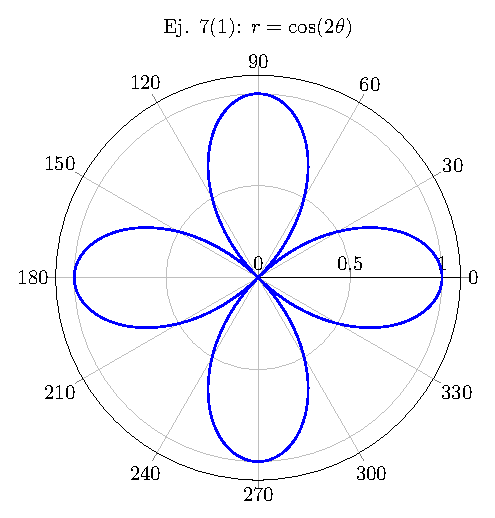
\includegraphics[width=0.4\textwidth]{Ej7 1.pdf}
    \end{figure}
    \item Por la imparidad del seno, afirmamos que $\sin(2(-\theta))=-\sin(2\theta)$. Así, los puntos de la función tales que $\theta \in [-\pi/2,\pi/2]$ están reflejados en el $[\pi/2,3\pi/2]$. Así, analizaremos los valores de $\theta$
    en el primer intervalo. Los valores de la función para $\theta=-\pi/2,-\pi/3,-\pi/6,0,\pi/6,$ $\pi/3,\pi/2$ son $0,-\sqrt{3}/2,-\sqrt{3}/2,0,\sqrt{3}/2,\sqrt{3}/2,0$ respectivamente.
    \begin{figure}[H]
        \centering
        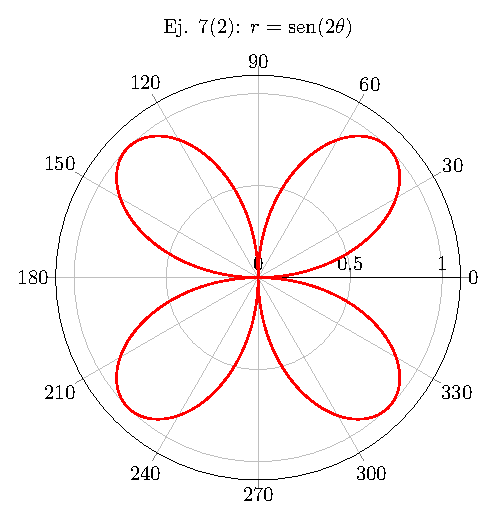
\includegraphics[width=0.4\textwidth]{Ej7 2.pdf}
    \end{figure}
    $\hfill \blacktriangle$
\end{enumerate}

\item Bosqueja las gr\'aficas de las siguientes funciones en el plano $xy$:
\begin{enumerate}[(1)]
\item $r=\sen(3\theta)$.
\item $r=\cos(3\theta)$.
\end{enumerate}
\textbf{Solución.}
\begin{enumerate}[(1)]
    \item Por la imparidad del seno, afirmamos que $\sin(3(-\theta))=-\sin(3\theta)$. Así, los puntos de la función tales que $\theta \in [-\pi/2,\pi/2]$ están reflejados en el $[\pi/2,3\pi/2]$. Así, analizaremos los valores de $\theta$
    en el primer intervalo. Los valores de la función para $\theta=-\pi/2,-\pi/3,-\pi/6,0,\pi/6,$ $\pi/3,\pi/2$ son $1,0,-1,0,1,0,-1$ respectivamente.
    \begin{figure}[H]
        \centering
        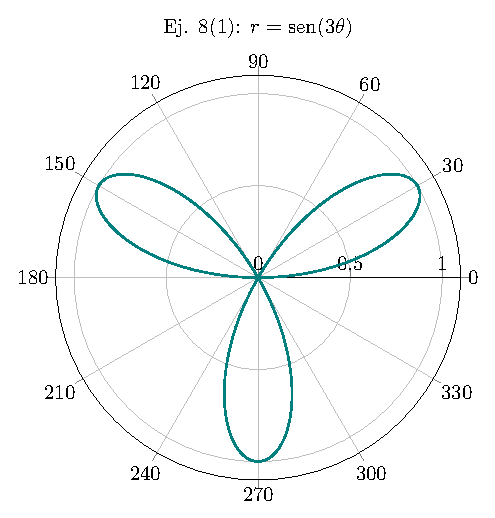
\includegraphics[width=0.4\textwidth]{Ej8 1.pdf}
    \end{figure}
    \item Puesto que $\cos(3(-\theta))=\cos(3\theta)$, afirmamos que los puntos tales que $\theta \in [\pi,2\pi]$ son un reflejo de los puntos en $[0,\pi]$. Así, basta analizar la gráfica para dichos valores de $\theta$.
    Señalamos que los valores de la función para $\theta=0,\pi/6,\pi/3,\pi/2,2\pi/3,5\pi/6,\pi$ son $1,0,-1,0,1,0,-1$ respectivamente.
    \begin{figure}[H]
        \centering
        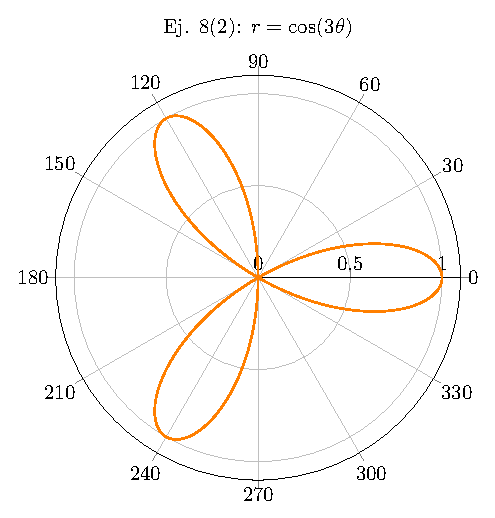
\includegraphics[width=0.4\textwidth]{Ej8 2.pdf}
    \end{figure}
    $\hfill \blacktriangle$
\end{enumerate}

\newpage
\item Bosqueja las superficies descritas en coordenadas cil\'indricas por:
\begin{enumerate}[(1)]
\item $r=3$.
\item $r=\cos(2\theta)$.
\end{enumerate}
\textbf{Solución.}
\begin{enumerate}[(1)]
    \item Por el ejercio 10, sabemos que $r=3$ describe a la circunferencia de radio 3. Así, la superficie descrita es la de la cáscara de un cilindro sin tapas.
    \begin{figure}[H]
        \centering
        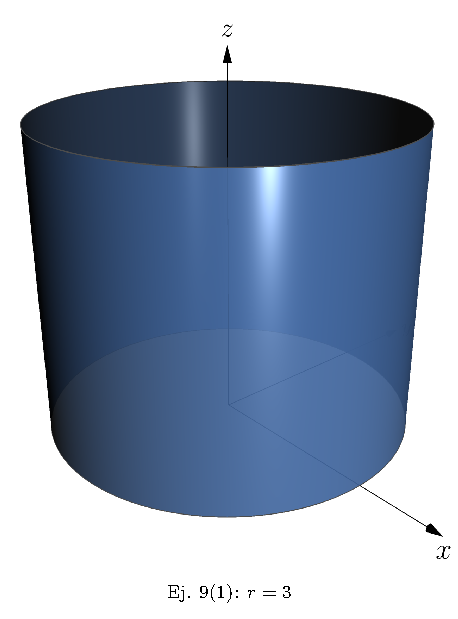
\includegraphics[width=.25\textwidth]{cilindricas1(alternativa).pdf}
    \end{figure}
    \item Es la superficie genereda al trasladar sobre el eje $z$ la gráfica descrita en el ejercicio 7, inciso (1).
    \begin{figure}[H]
        \centering
        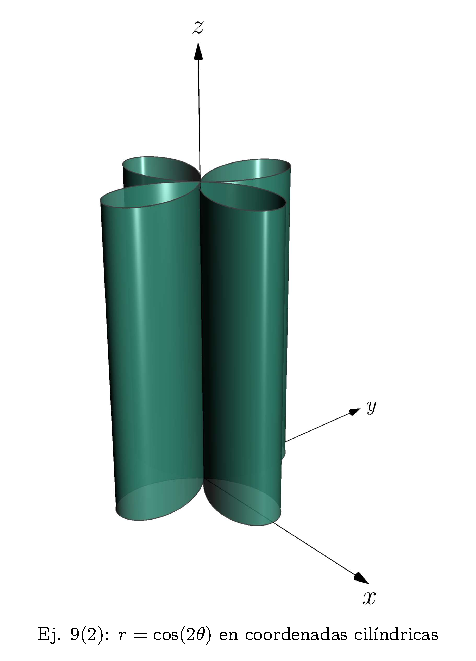
\includegraphics[width=0.4\textwidth]{cilindricas2(alternativas).pdf}
    \end{figure}
\end{enumerate}

\newpage
\item Describe las ecuaciones de las c\'onicas en coordenadas polares. \\
\textbf{Demostración.} Sea $(r,\theta)\in \R^2_{r,\theta}$ un punto en la circunferencia con centro en el origen de radio $t$. Tomando la representación de $(r,\theta)$ en
$\R^2$, y la ecuación de la circunferencia en dichas coordenadas, tenemos que
\begin{align*}
    (r\cos\theta)^2+(r\sin\theta)^2=t^2 &\iff r^2(\cos^2\theta+\sin^2\theta)=t^2 \\
    &\iff r^2=t^2
\end{align*}
y puesto que tanto $t$ como $r$ son números positivos, concluimos que la ecuación es $r=t$. Para el caso de la elipse horizontal de parámetros $a,b$ con centro en el origen obtenemos que
\begin{align*}
    \frac{(r\cos\theta)^2}{a^2}+\frac{(r\sin\theta)^2}{b^2}=1 &\iff r^2\left(\frac{\cos^2\theta}{a^2}+\frac{\sin^2\theta}{b^2}\right)=1\\
    &\iff r^2\left(\frac{b^2\cos^2\theta+a^2\sin^2\theta}{a^2b^2}\right)=1 \\
    &\iff r^2=\frac{a^2b^2}{b^2\cos^2\theta+a^2\sin^2\theta}.
\end{align*}
De ser la elipse vertical, se intercambian de lugar las constantes $a$ y $b$ en la ecuación anterior. Veámos el caso de la hipérbola horizontal de parámetros $a,b$ y centro en el origen. Tenemos que
\begin{align*}
    \frac{(r\cos\theta)^2}{a^2}-\frac{(r\sin\theta)^2}{b^2}=1 &\iff r^2\left(\frac{\cos^2\theta}{a^2}-\frac{\sin^2\theta}{b^2}\right)=1\\
    &\iff r^2\left(\frac{b^2\cos^2\theta-a^2\sin^2\theta}{a^2b^2}\right)=1 \\
    &\iff r^2=\frac{a^2b^2}{b^2\cos^2\theta-a^2\sin^2\theta}.
\end{align*}
Si se trata de una hipérbola con los mismos parámetros, pero horizontal, obtenemos que
\begin{align*}
    \frac{(r\sin\theta)^2}{a^2}-\frac{(r\cos\theta)^2}{b^2}=1 &\iff r^2\left(\frac{\sin^2\theta}{a^2}-\frac{\cos^2\theta}{b^2}\right)=1\\
    &\iff r^2\left(\frac{b^2\sin^2\theta-a^2\cos^2\theta}{a^2b^2}\right)=1 \\
    &\iff r^2=\frac{a^2b^2}{b^2\sin^2\theta-a^2\cos^2\theta}.
\end{align*}
Resta la parábola. De ser una parábola horizontal de parámetro $p$ con centro en el origen, se tiene que
\begin{align*}
    (r\sin\theta)^2=4p\cos\theta &\iff r^2\sin^2\theta = 4p\cos\theta \\
    &\iff r^2 = \frac{4p\cos\theta}{\sin^2\theta}.
\end{align*}
Finalmente, de tratarse de una parábola vertical (nuevamente con parámetro $p$) se sigue que
\begin{align*}
    (r\cos\theta)^2=4p\sin\theta &\iff r^2\cos^2\theta = 4p\sin\theta \\
    &\iff r^2 = \frac{4p\sin\theta}{\cos^2\theta}.    \quad \blacksquare
\end{align*}
\end{enumerate}

\end{document}
